\documentclass[12pt,a4paper,oneside]{article}

% --- Paquets bàsics ---
\usepackage[utf8]{inputenc}
\usepackage[T1]{fontenc}
\usepackage[provide=*]{babel} 
\babelprovide[main, import]{catalan}
\usepackage{graphicx}
\usepackage{geometry}
\geometry{a4paper, margin=2.5cm}
\usepackage{setspace}
\setstretch{1.3}

% --- Tipografia Moderna ---
\usepackage[default]{sourcesanspro}
\renewcommand{\familydefault}{\sfdefault}
\usepackage{microtype} 

% --- Disseny i Colors ---
\usepackage[dvipsnames, table]{xcolor}
\usepackage{listings}
\usepackage{tcolorbox}
\tcbuselibrary{skins} 
\usepackage{titlesec}
\usepackage{enumitem}
\usepackage{tikz} 
\usetikzlibrary{shapes.geometric, arrows, positioning, shadows}

% --- DEFINICIÓ DE COLORS ---
\definecolor{MainBlue}{HTML}{003366}

% Configurem hyperref perquè els enllaços tinguin color i no recuadres lletjos
\usepackage[colorlinks=true, linkcolor=MidnightBlue, urlcolor=TealBlue, citecolor=RoyalBlue]{hyperref} 

% --- Disseny de l'Índex ---
\usepackage{tocloft}
\renewcommand{\cftsecleader}{\cftdotfill{\cftdotsep}} 
\renewcommand{\cftsecfont}{\bfseries\color{MidnightBlue}} 
\renewcommand{\cftsubsecfont}{\small\color{RoyalBlue}} 
\setlength{\cftbeforesecskip}{8pt} 

% --- Capçaleres i Peus de pàgina ---
\usepackage{fancyhdr}
\setlength{\headheight}{25pt}
\pagestyle{fancy}
\fancyhf{} 
\renewcommand{\headrulewidth}{0.6pt}
\renewcommand{\headrule}{\hbox to\headwidth{\color{MidnightBlue}\leaders\hrule height \headrulewidth\hfill}}
\fancyhead[L]{\small\color{gray} Laia Cabrera Vallejos} 
\fancyhead[R]{\small\color{MidnightBlue} \nouppercase{\leftmark}} 
\fancyfoot[R]{\thepage}

% --- Configuració de peus de figura ---
\usepackage[labelfont=bf, font=small, skip=10pt]{caption}

% --- Elements Gràfics Addicionals ---
\usepackage{booktabs} 
\usepackage{pifont} 
\newcommand{\cmark}{\ding{51}}%
\newcommand{\xmark}{\ding{55}}%

% --- Maquetació de Títols ---
\titleformat{\section}[block]
  {\normalfont\Huge\bfseries\color{MidnightBlue}}{}{0pt}{}
\titlespacing*{\section}{0pt}{10pt}{20pt}

\titleformat{\subsection}[block]
  {\normalfont\Large\bfseries\color{RoyalBlue}}{}{0pt}{}
\titlespacing*{\subsection}{0cm}{18pt}{10pt}

% --- Comanda per a salts de pàgina intel·ligents (Regla del 75%) ---
\usepackage{needspace}
\newcommand{\apartat}[1]{\needspace{0.25\textheight}\section{#1}}

% ---------------------------------------------------------
% INICI DEL DOCUMENT
% ---------------------------------------------------------
\begin{document}

% --- PORTADA FINAL (GARANTIA PÀGINA ÚNICA) ---
\begin{titlepage}
    \begin{tikzpicture}[remember picture,overlay]
        % Marc blau exterior
        \draw[line width=1.5pt, color=MidnightBlue] 
            ([xshift=0.8cm,yshift=-0.8cm]current page.north west) 
            rectangle 
            ([xshift=-0.8cm,yshift=0.8cm]current page.south east);
            
        % Logo a la cantonada superior dreta
        \node[anchor=north east, xshift=-1.2cm, yshift=-1.2cm] at (current page.north east) 
            {
\includegraphics[width=2.1cm]{imatges/logo_intitut.png}};
            
        % Text Institut a dalt a l'esquerra
        \node[anchor=north west, xshift=1.2cm, yshift=-1.5cm] at (current page.north west) 
            {\small \textbf{INSTITUT ESCOLA SANT POL DE MAR}};
    \end{tikzpicture}

    \centering
    \vspace*{3.5cm}

    \begin{tcolorbox}[colback=white, colframe=MidnightBlue, arc=5pt, boxrule=1.5pt, left=1cm, right=1cm, top=1cm, bottom=1cm, shadow={4pt}{-4pt}{0pt}{black!15}]
        \centering
        {\Huge \textbf{\color{MidnightBlue} LA COMUNICACIÓ A TRAVÉS\\ DELS SENTITS}} \par
        \vspace{0.6cm}
        {\Large \textit{Disseny i utilitat d'una taula sensorial per a persones amb dificultats comunicatives}}
    \end{tcolorbox}

    \vspace{1.5cm}
    \begin{tcolorbox}[colback=white, colframe=gray!5, arc=15pt, width=12cm, boxrule=0.2pt, halign=center, shadow={2pt}{-2pt}{0pt}{black!5}]
        \centering
        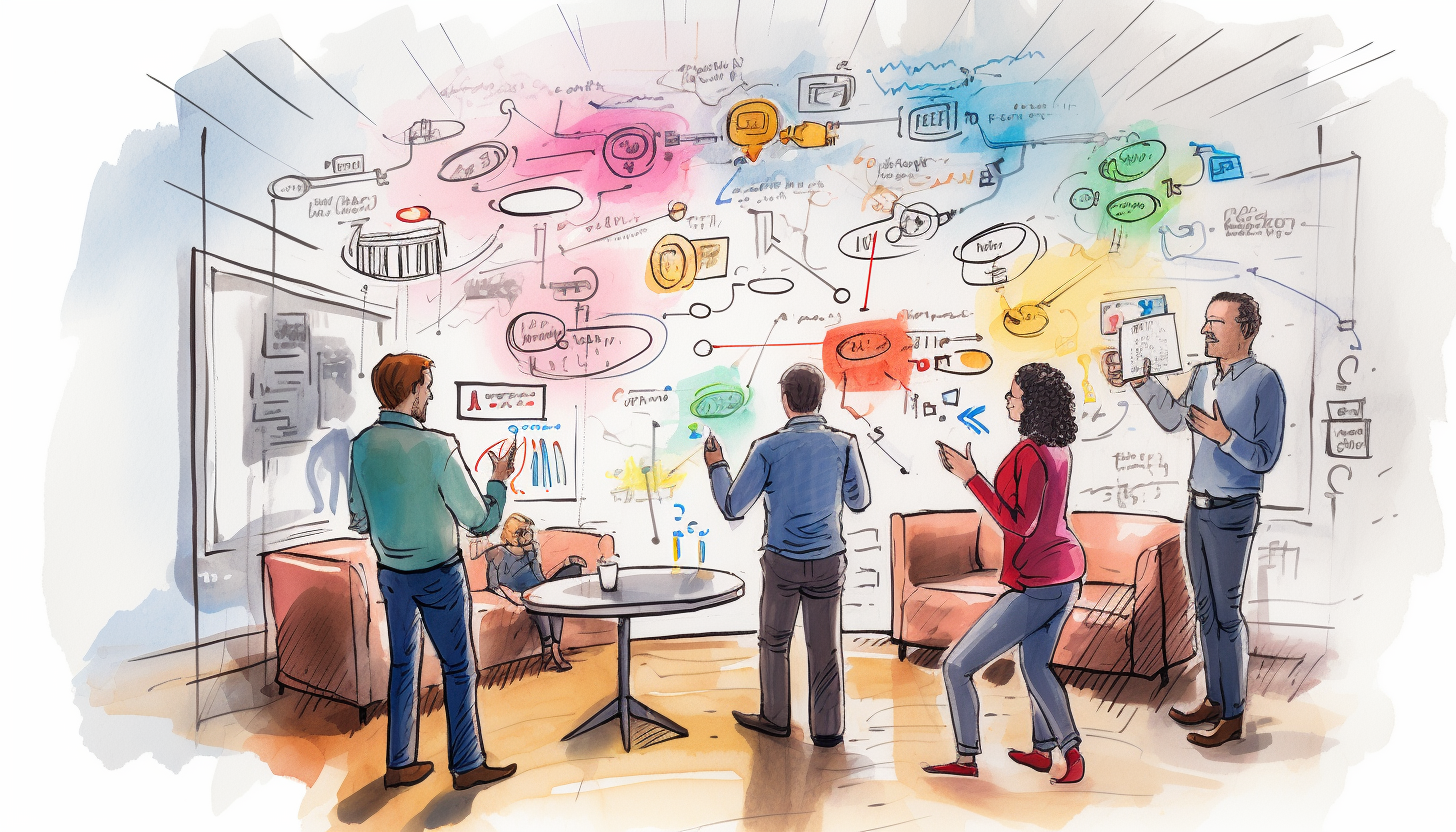
\includegraphics[width=11.5cm]{imatges/dibuix_que-representa-un-grup-de-presonse-comunicant-se-i-expresant-les-seves-idees-parlant-i-atraves-d'esquemes.png}
    \end{tcolorbox}

    \vfill

    \begin{minipage}{0.8\textwidth}
        \centering
        \textbf{\large Treball de Recerca de Batxillerat} \\
        \textsf{Curs 2025-2026}
    \end{minipage}

    \vspace{1.2cm}

    \begin{minipage}[t]{0.4\textwidth}
        \begin{flushleft} 
            \textsc{Autora:}\\
            \textbf{Laia Cabrera Vallejos}
        \end{flushleft}
    \end{minipage}
    \begin{minipage}[t]{0.4\textwidth}
        \begin{flushright}
            \textsc{Tutor:}\\
            \textbf{Enric Abadal Maestro}
        \end{flushright}
    \end{minipage}

    \vspace{0.3cm}
\end{titlepage}

% --- ÍNDEX ---
\pagenumbering{Alph}
\hypersetup{pageanchor=false}
{\color{MidnightBlue}\tableofcontents}
\newpage
\pagenumbering{arabic}
\setcounter{page}{1}
\hypersetup{pageanchor=true}

% --- SECCIÓ 1: INTRODUCCIÓ ---
\apartat{Introducció i Motivació}

\subsection{Motius de la tria del projecte}
La comunicació és un dret fonamental de tot ésser humà. No obstant això, per a moltes persones, aquest procés que la majoria realitzem de manera instintiva es converteix en una barrera infranquejable. La motivació principal d'aquest treball neix de la voluntat d'entendre i mitigar la frustració que senten aquelles persones que tenen idees, desitjos i emocions, però que no disposen dels canals adequats per expressar-los.

A nivell personal, l'interès neix d'observar com petits canvis en l'entorn poden transformar completament la interacció d'una persona amb el seu món. La taula sensorial és una eina que, tot i la seva aparent simplicitat física, amaga una gran complexitat de disseny pedagògic i terapèutic.

\begin{figure}[ht]
    \centering
    \begin{tcolorbox}[colback=white, colframe=MidnightBlue!20, arc=5pt, boxrule=0.5pt, left=2pt, right=2pt, top=2pt, bottom=2pt, shadow={1pt}{-1pt}{0pt}{black!5}]
        \centering
        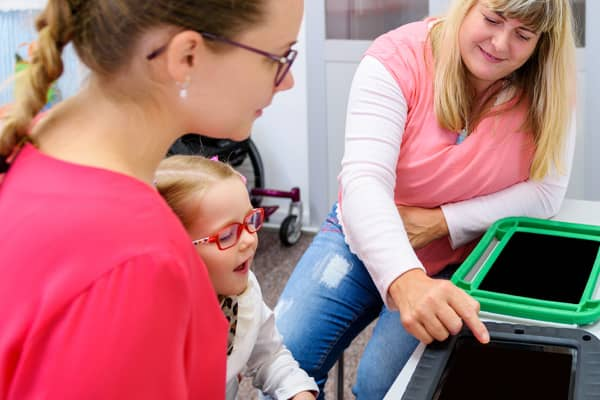
\includegraphics[width=0.8\textwidth]{imatges/persona-adulta-ensenyant-la-taula-de-neuroKids-per-la-communicacio-no-verbal-a-una-jove-i-una-nena-petita.jpg}
    \end{tcolorbox}
    \caption{Interacció multisensorial: l'espai com a facilitador de vincles afectius i aprenentatge social.}
    \label{fig:interaccio_sensorial}
\end{figure}

\newpage
\subsection{Orientació i objectius del treball}
Aquest projecte s'orienta des d'una perspectiva holística\footnote{Enfocament que considera la persona com un tot, integrant aspectes físics, psicològics i socials.}. L'enfocament es divideix en quatre eixos:
\begin{itemize}
    \item \textbf{Inclusió real:} Creació d'entorns accessibles per a tothom, potenciant l'autodeterminació\footnote{Capacitat de la persona per ser l'agent causal de la seva pròpia vida i prendre decisions sense influències externes indegudes.}.
    \item \textbf{Perspectiva logopèdica:} Reforç de les estructures del llenguatge mitjançant estímuls paral·lels.
    \item \textbf{Educació especial:} Proposta de materials tangibles per al suport a l'aula.
    \item \textbf{Impacte en la vida diària:} Solucions pràctiques per a l'entorn familiar.
\end{itemize}

\subsection{La importància de la diversitat en la societat actual}
Vivim en un món que a poc a poc va entenent que la diversitat no és un problema a resoldre, sinó un valor a integrar. Malgrat aquest avanç, encara trobem "deserts comunicatius"\footnote{Entorns on les persones amb dificultats no troben cap suport ni interlocutor preparat per entendre els seus mètodes alternatius de comunicació.} que cal abordar des de la innovació i el disseny inclusiu.

% --- SECCIÓ 3: OBJECTIUS I HIPÒTESI ---
\apartat{Objectius i Hipòtesi}

\subsection{Objectius del Projecte}
El present treball es proposa assolir una sèrie de fites tant teòriques com pràctiques:
\begin{itemize}
    \item \textbf{Objectiu 1:} Analitzar les bases científiques de la comunicació no verbal i la seva importància en el desenvolupament humà.
    \item \textbf{Objectiu 2:} Estudiar el funcionament dels sistemes de Comunicació Augmentativa i Alternativa (CAA) actuals.
    \item \textbf{Objectiu 3:} Dissenyar i construir un prototip funcional de taula sensorial que integri estímuls tàctils, visuals i sonors.
    \item \textbf{Objectiu 4:} Avaluar la utilitat de la taula com a eina de suport per a col·lectius amb necessitats especials.
\end{itemize}

\newpage
\subsection{Hipòtesi de Recerca}
La hipòtesi principal que guia aquest treball és la següent:
\begin{quote}
    \textit{"L'ús d'una taula sensorial dissenyada específicament per a l'estimulació multisensorial facilita la intenció comunicativa i millora la capacitat d'expressió de les persones amb dificultats greus en la parla."}
\end{quote}

Aquesta hipòtesi se sustenta en la teoria de la integració sensorial, que defensa que un cervell ben regulat sensorialment és més capaç de processar informació social complexa.

% --- SECCIÓ 2: MARC TEÒRIC ---
\apartat{Marc Teòric}

\subsection{La Comunicació Humana i el seu Processament}
La comunicació és un procés complex i multidimensional que permet als éssers humans intercanviar informació, expressar emocions i construir relacions socials. Des d'una perspectiva neuropsicològica, la comunicació requereix la integració de múltiples àrees cerebrals, especialment l'àrea de Broca i l'àrea de Wernicke\footnote{L'àrea de Broca s'encarrega de la producció del llenguatge, mentre que l'àrea de Wernicke és fonamental per a la comprensió del mateix.}, que gestionen tant el contingut com la forma del missatge.

% --- ESQUEMA TÈCNIC: COMPONENTS DE LA COMUNICACIÓ ---
\begin{figure}[ht]
    \centering
    \begin{tikzpicture}[node distance=1.5cm, auto,
        block/.style={rectangle, draw, fill=MidnightBlue!10, text width=8em, text centered, rounded corners, minimum height=3.5em, font=\small, drop shadow},
        line/.style={draw, -latex', MidnightBlue, thick}]
        
        \node [block, fill=MidnightBlue!25] (com) {\textbf{Estructura de la Comunicació}};
        \node [block, below left=1.5cm and 0.2cm of com] (verb) {Component Verbal\\(Semàntica i Sintaxi)};
        \node [block, below=2cm of com] (noverb) {Component No Verbal\\(Cinèsica i Proxèmica)};
        \node [block, below right=1.5cm and 0.2cm of com] (caa) {CAA\\(Suport Multimodal)};
        
        \path [line] (com) -- (verb);
        \path [line] (com) -- (noverb);
        \path [line] (com) -- (caa);
    \end{tikzpicture}
    \caption{Representació gràfica de les dimensions comunicatives abordades en el treball.}
\end{figure}

\newpage
\subsection{Comunicació Augmentativa i Alternativa (CAA)}
\begin{tcolorbox}[colback=TealBlue!5, colframe=TealBlue, arc=5pt, title=La CAA com a eina d'inclusió, fonttitle=\bfseries, shadow={2pt}{-2pt}{0pt}{black!10}]
    La CAA engloba tot aquell conjunt d'estratègies que busquen maximitzar les capacitats comunicatives. Segons l'ISAAC\footnote{International Society for Augmentative and Alternative Communication.}, l'objectiu no és només parlar, sinó permetre la participació plena en la societat.
\end{tcolorbox}

% --- TAULA COMPARATIVA DE SISTEMES ---
\begin{table}[ht]
    \centering
    \small
    \begin{tabular}{@{} l p{3.5cm} c c c @{}}
    \toprule
    \textbf{Sistema} & \textbf{Descripció} & \textbf{Portabilitat} & \textbf{Càrrega Cognitiva} & \textbf{Autonomia} \\
    \midrule
    \rowcolor{gray!5} ARASAAC & Pictogrames gratuïts & \cmark & Baixa & Alta \\
    SPC & Símbols clàssics & \cmark & Baixa & Mitjana \\
    \rowcolor{gray!5} DCOV & Dispositius amb veu & \xmark & Alta & Molt Alta \\
    \bottomrule
    \end{tabular}
    \caption{Anàlisi comparatiu de les solucions de suport segons criteris tècnics.}
\end{table}

\subsection{Integració Sensorial: Fonaments i Impacte}
La integració sensorial és el procés neurològic d'organitzar les sensacions per al seu ús. Segons la piràmide d'aprenentatge de Williams i Shellenberger\footnote{Model que explica com el desenvolupament sensorial és la base de les habilitats cognitives i acadèmiques.}, la regulació dels sentits és el fonament de tot creixement acadèmic.

% --- ESQUEMA TIKZ: PIRÀMIDE SENSORIAL ---
\begin{figure}[ht]
    \centering
    \begin{tikzpicture}[scale=0.8]
        \draw[thick, fill=MidnightBlue!5] (0,0) -- (6,0) -- (3,5) -- cycle;
        \draw[MidnightBlue] (0.6,1) -- (5.4,1);
        \draw[MidnightBlue] (1.2,2) -- (4.8,2);
        \draw[MidnightBlue] (1.8,3) -- (4.2,3);
        
        \node at (3,0.5) {\footnotesize\textbf{Sistemes Sensorials} (Base)};
        \node at (3,1.5) {\footnotesize Desenvolupament Sensoriomotor};
        \node at (3,2.5) {\footnotesize Percepció Perceptivomotora};
        \node at (3,3.8) {\footnotesize\textbf{Aprenentatge}};
    \end{tikzpicture}
    \caption{Piràmide simplificada de la integració sensorial en el desenvolupament.}
\end{figure}

La taula sensorial actua en la base d'aquesta piràmide, oferint estímuls tàctils i visuals que preparen el cervell per a processos superiors com el llenguatge.

\subsection{Dificultats Comunicatives Específiques}
\begin{itemize}
    \item \textbf{TEA (Trastorn de l'Espectre Autista):} Presenten dificultats en la comunicació social. La regulació sensorial mitjançant llums i textures pot reduir l'estrès ambiental.
    \item \textbf{Paràlisi Cerebral:} Afecta l'execució motora. La taula sensorial ofereix una via d'interacció que no depèn de la motricitat fina.
    \item \textbf{Retard maduratiu:} L'estimulació multisensorial accelera la creació de connexions neuronals (neuroplasticitat).
\end{itemize}

% --- SECCIÓ 4: METODOLOGIA ---
\apartat{Metodologia de Recerca}
El rigor científic d'aquest treball es fonamenta en una metodologia de tall qualitatiu i experimental, adaptada a la naturalesa humana i tecnològica del projecte.

% --- ESQUEMA DE FLUX DE METODOLOGIA ---
\begin{figure}[ht]
    \centering
    \begin{tikzpicture}[node distance=1cm, auto,
        metstep/.style={rectangle, draw, fill=RoyalBlue!10, text width=12cm, text centered, rounded corners, minimum height=2.5em, font=\small, drop shadow},
        arrow/.style={thick,->,>=stealth, RoyalBlue}]
        
        \node [metstep] (s1) {\textbf{Fase 1: Diagnòstic} \\ Identificació de barreres comunicatives.};
        \node [metstep, below=of s1] (s2) {\textbf{Fase 2: Validació Externa} \\ Entrevistes a professionals de la Fundació Horitzó.};
        \node [metstep, below=of s2] (s3) {\textbf{Fase 3: Disseny Tècnic} \\ Selecció d'estímuls i planificació ergonòmica.};
        \node [metstep, below=of s3] (s4) {\textbf{Fase 4: Realització Física} \\ Construcció del prototip funcional.};
        \node [metstep, below=of s4] (s5) {\textbf{Fase 5: Avaluació} \\ Recollida d'evidències d'ús.};
        
        \draw [arrow] (s1) -- (s2);
        \draw [arrow] (s2) -- (s3);
        \draw [arrow] (s3) -- (s4);
        \draw [arrow] (s4) -- (s5);
    \end{tikzpicture}
    \caption{Full de ruta metodològic del projecte.}
\end{figure}

\subsection{Disseny i Desenvolupament del Prototip}
\begin{enumerate}
    \item \textbf{Recerca de referents:} Anàlisi d'espais Snoezelen\footnote{Sales de relaxació i estimulació multisensorial.} per triar els colors i textures més efectius.
    \item \textbf{Selecció de materials:} Ús de components segurs (fustes polides, LEDs de 12V, textures naturals com suro i lli).
    \item \textbf{Verificació d'usabilitat:} Proves de pressió per assegurar que qualsevol usuari pot interactuar amb la taula sense esforç excessiu.
\end{enumerate}

\begin{figure}[ht]
    \centering
    \begin{tcolorbox}[colback=white, colframe=RoyalBlue!20, arc=5pt, boxrule=0.5pt, left=2pt, right=2pt, top=2pt, bottom=2pt, shadow={1pt}{-1pt}{0pt}{black!5}]
        \centering
        
\includegraphics[width=0.8\textwidth]{imatges/Overcoming-Language-Barriers-Enhancing-Communication-Skills-in-a-Multicultural-Workplace-with-Hospitality-tecles_d'ordinador_amb-diferents_banderes_de_diferents_païssos_amb_el_botó_de_translate_al_mitg.png}
    \end{tcolorbox}
    \caption{La tecnologia com a pont universal per superar barreres comunicatives.}
\end{figure}

% --- SECCIÓ 5: CONCLUSIONS ---
\apartat{Conclusions}
Aquest treball ha permès aprofundir en la relació intrínseca entre la percepció sensorial i la capacitat comunicativa humana. Les conclusions principals s'estructuren segons els resultats obtinguts:

\begin{itemize}
    \item \textbf{Facilitació del llenguatge:} S'ha confirmat que els sistemes de comunicació augmentativa (CAA) actuen com un pont que potencia, en lloc de frenar, el desenvolupament de la intenció comunicativa.
    \item \textbf{Regulació sensorial:} Els estímuls controlats de la taula sensorial són eficaços per focalitzar l'atenció de l'usuari i reduir l'estrès ambiental, creant un estat òptim per a l'aprenentatge.
    \item \textbf{Autonomia i Empoderament:} La interacció directa amb la taula millora l'autoconcepte de l'usuari en veure que les seves accions tenen una resposta sensorial immediata i predictible.
\end{itemize}

En definitiva, la comunicació a través dels sentits és una eina clau per garantir la plena inclusió i dignitat de totes les persones en la nostra societat.

% --- BIBLIOGRAFIA ---
\apartat{Bibliografia i Webgrafia}
\markboth{Bibliografia i Webgrafia}{}
\addcontentsline{toc}{section}{Bibliografia i Webgrafia}

\begin{description}[style=unboxed, leftmargin=0cm, itemsep=1.2em]
    \sloppy
    \raggedright

    \item[ARASAAC.] (s.d.). \textit{¿Qué es la comunicación aumentativa y alternativa?}. Centro Aragonés para la Comunicación Aumentativa y Alternativa. \url{https://arasaac.org/aac/es}

    \item[American Speech-Language-Hearing Association (ASHA).] (2021). \textit{Augmentative and Alternative Communication (AAC)}. \url{https://www.asha.org/public/speech/disorders/aac/}

    \item[Beukelman, D. R., \& Light, J. C.] (2020). \textit{Augmentative and Alternative Communication: Supporting Children and Adults with Complex Communication Needs} (5th ed.). Paul H. Brookes Publishing Co.

    \item[Institut Obert de Catalunya.] (s.d.). \textit{Atenció a la comunicació}. Materials del cicle formatiu d'Atenció a Persones en Situació de Dependència. \url{https://ioc.xtec.cat/materials/FP/Recursos/fp_apd_m09_/web/fp_apd_m09_htmlindex/WebContent/u1/a1/continguts.html}

    \item[Mayo Clinic.] (2023). \textit{Autism spectrum disorder - Symptoms and causes}. \url{https://www.mayoclinic.org/diseases-conditions/autism-spectrum-disorder/symptoms-causes/syc-20352928}

    \item[Pagliano, P.] (2012). \textit{The Multisensory Handbook: A Guide for Children and Adults with Sensory Learning Disabilities}. Routledge.

    \item[Sensory Processing Disorder Foundation.] (2024). \textit{About SPD: Sensory Processing Disorder}. \url{https://www.spdstar.org/basic/about-spd}

    \item[UNESCO.] (2020). \textit{Towards inclusion in education: status, trends and challenges}. \url{https://unesdoc.unesco.org/ark:/48223/pf0000373844}

\end{description}


\end{document}
